\documentclass[12pt, twocolumn, x11names]{article}

\usepackage{amsmath}
\usepackage{hyperref}
\usepackage{graphicx}
\usepackage{tikz}
\usepackage{booktabs}
\usepackage{caption}
\usepackage{subcaption}
\usepackage{epigraph}
\usepackage{multirow}
\captionsetup[figure]{font=small}
\captionsetup[table]{font=small}
\captionsetup[subfigure]{font=scriptsize}

%% \usepackage{microtype}
\usepackage{sectsty}
\sectionfont{\bfseries \normalsize \uppercase}
\subsectionfont{\normalsize}
\subsubsectionfont{\normalsize \normalfont \itshape}


% \usepackage{multicol}
\setlength{\columnsep}{0.5cm}
\setlength{\parskip}{0pt}

\usepackage[a4paper, total={7in,9in}]{geometry}

% MOM stop splitting the footnotes
\interfootnotelinepenalty=10000

\usepackage{natbib}
\bibliographystyle{ametsoc2014}
%\usepackage[maxcitenames=3, maxbibnames=3, style=ametsoc2014.bst, backend=biber, natbib=true]{biblatex}
%% \setcitestyle{authoryear}
%% \AtEveryBibitem{\clearfield{month}}
%% \AtEveryBibitem{\clearfield{day}}
%% \AtEveryBibitem{\clearfield{isbn}}
%% \AtEveryBibitem{\clearfield{issn}}
%% \AtEveryBibitem{\clearfield{doi}}
%% \AtEveryBibitem{\clearfield{url}}
%% \AtEveryBibitem{\clearfield{eprint}}


\newcommand{\elnino}[0]{\emph{El Ni\~no}}
\newcommand{\enso}[0]{\emph{ENSO}}
\newcommand{\nina}[0]{\emph{La Ni\~na}}
\newcommand{\degc}{^{\circ}\mathrm{C}}

% TODO A better title. Something witty and fun.
%% \title{\elnino{} and Africa}
%% \author{Luke Conaboy and Mark G. Skilbeck}
%% \date{}

\usepackage[pages=some]{background}
\backgroundsetup{
scale=1,
color=black,
opacity=1 ,
angle=0,
placement=top,
contents={%
  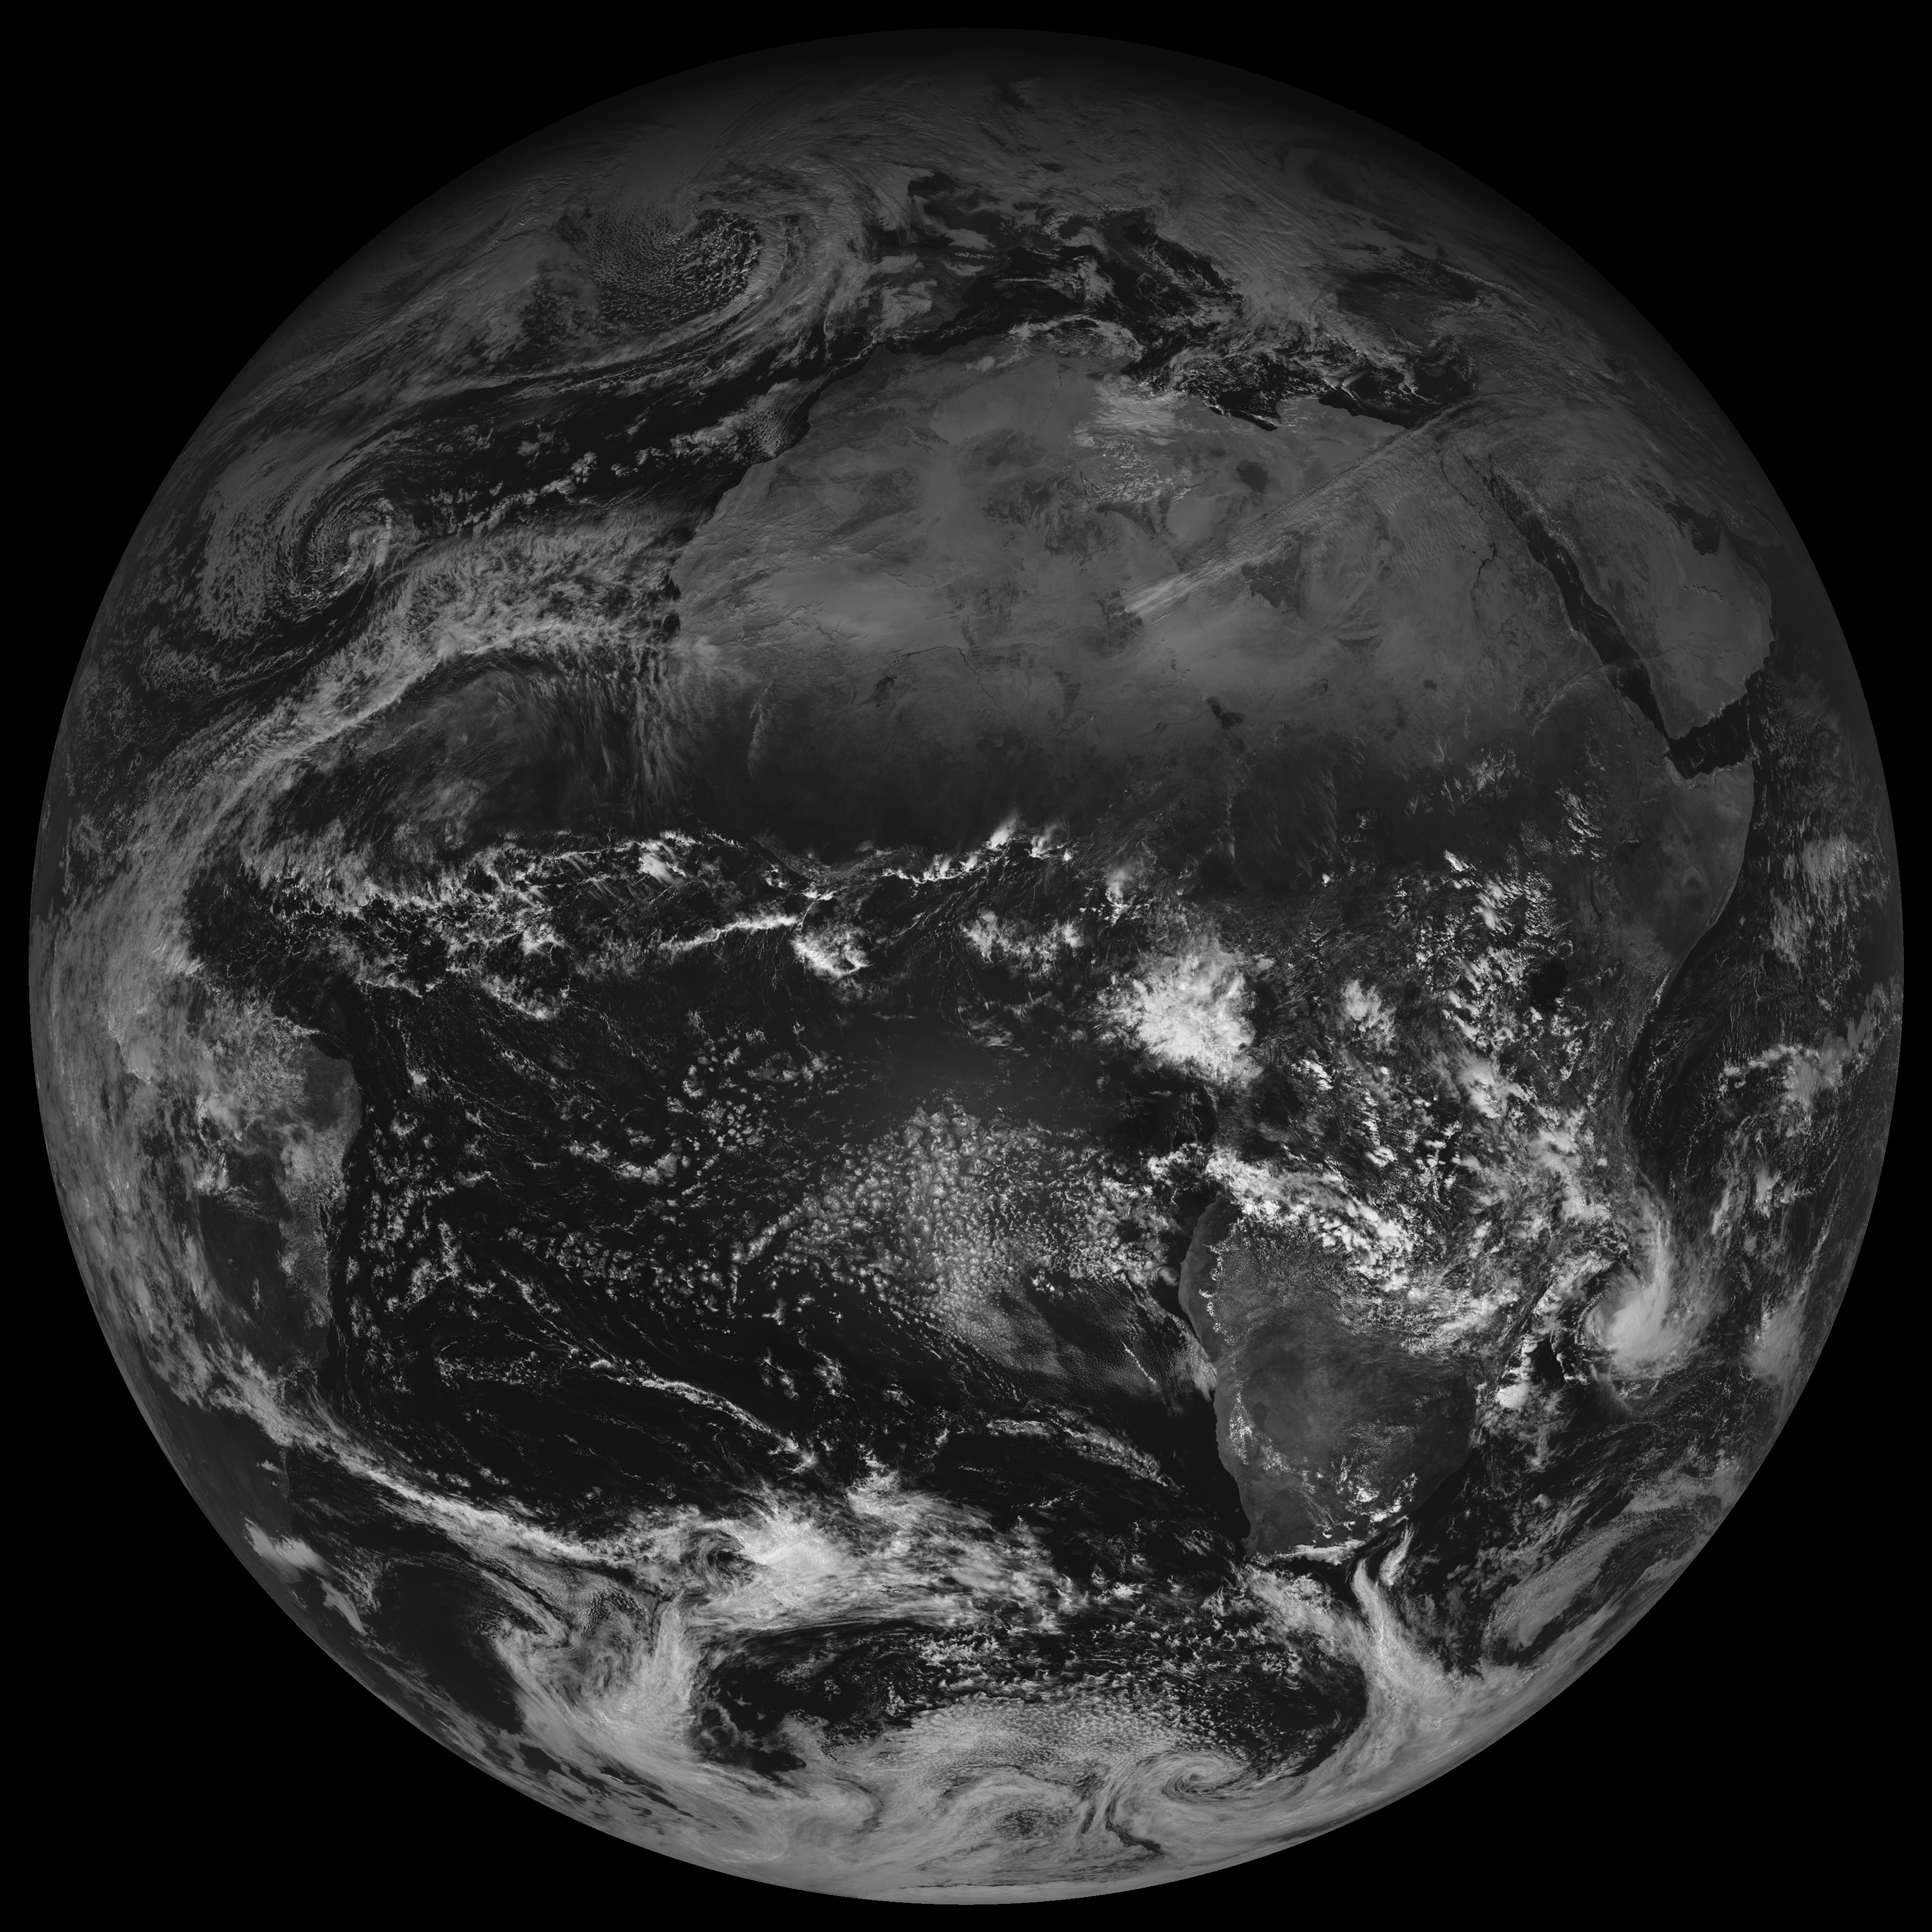
\includegraphics[width=\paperwidth,height=\paperwidth]{figures/image.png}
  }%
}

\usepackage{geometry}

% Hacky. On the page with the pixel distributions, putting both
% figures on a single page makes the texr overflow onto the page
% number. Haven't found a good way to move the page number for a
% single page, so this moves page number for every page.
\setlength{\footskip}{1in}

\begin{document}

%% \twocolumn[
%%   \begin{@twocolumnfalse}
%%     \maketitle
%%     \begin{abstract}
%%       This is driving me to abstraction
%%     \end{abstract}
%%   \end{@twocolumnfalse}
%% ]

\begin{titlepage}
  \begin{center}
    \includegraphics[width=0.33\textwidth]{figures/uon_logo}
    \vspace{3cm}
    
    \textsf{\textbf{\Huge \elnino{} and Africa}} \\ 
    \vspace{2cm}
           {\Large Luke Conaboy and Mark G. Skilbeck} \\
           \vspace{1cm}
           {\Large\today}
           \vspace{2cm}
    \begin{abstract}
      Fair.
    \end{abstract}
  \end{center}
\end{titlepage}

\newpage
\newgeometry{left=2cm, right=5cm, bottom=1cm, top=0cm}

\BgThispage
\thispagestyle{empty}

\vspace*{21cm}
\setlength\epigraphwidth{.8\textwidth}
\epigraph{\Huge I bless the rains down in Africa}{--- \emph{Africa}, Toto}

\restoregeometry

\clearpage
\setcounter{page}{1}

\section{Introduction}

The importance of weather forecasting cannot be understated. We regularly
consult weather forecasts to inform our clothing choices, to help us decide
whether a family outing should be a trip to the beach or to a museum; should we
bring along an umbrella? is it shirt-and-shorts weather?\footnote{Incidentally
  it is never \emph{shirt-and-\textbf{short}-shorts weather.}} These are
legitimate concerns, but they are decidedly \emph{first-world} concerns. In
parts of the world where the amount of rainfall literally means life or death it
is plainly obvious that forewarning of drought is of paramount importance.
Whereas wealthy nations may import food and water in times of need, much of
sub-Saharan Africa relies on the prosperity of local agriculture to meet dietary
needs. Any negative impact on the harvest -- here we concern ourselves only with
climatological causes -- will severely restrict available food sources
\citep{development2006mapping}. Modern Africa has been plagued by socioeconomic
struggles, with frequent civil war, little access to education and medicine, and
highly unstable governments. While much progress has been made in recent
years\footnote{For more information see \url{https://africaindata.org}} the
extra stresses of food shortages and drought may trigger a return to
instability.
% TODO Provide actual citation for above. Is the last line here a
% bit... insensitive?
In 2016 the UN Office for the Coordination of Humanitarian Affairs (UNOCHA)
published a report on the response to \elnino{} in East and Southern Africa
\citep{unocha2016}; by their estimates over 19.5 million people and 10.5
children were affected in East Africa alone. As a result of \elnino{} parts of
East Africa received below average rainfall leading to poor harvests and food
shortages. Similarly, parts of Southern Africa experienced the worst drought for
35 years and leading to huge food insecurity. As one of the worst hit countries,
Kenya alone now has over 1.2 million people in a food security crisis.

Malaria has long been a leading cause of death in Africa, particularly in
children, accounting for approximately 18\% of total deaths in children
\citep{IMHE2016}. \citet{alles1998} states that, at the time of reporting,
malaria transmission intensities---a measure of how effectively malaria is
transmitted in a population---are often two orders of magnitude greater than other
regions where malaria is a significant problem. \cite{loevinsohn1994}
investigated the relationship between climatic warming and malaria incidence
rates in Rwanda, East Africa. The report found that during the particularly warm
period of the late 1980s malaria incidence rates almost doubled, with even
regions previously free of the disease showing an up-take in
incidence.\footnote{Interestingly, the report notes that while there was no
  significant trend in precipitation over the same period, there was heavy rain
  in the years 1987 and 1988 which coincided with a strong ENSO event.}

More recently \cite{craig2004} sought to quantify the association between
various climatic factors---including rainfall and temperature---and malaria
incidence. The report found that \emph{total seasonal cases} of malaria were not
driven by climatological factors; however there was a strong correlation between
interseasonal variability and factors such as the maximum temperatures of the
preceeding season.


% For this reason, it is imperative that we improve our understand of and ability
% to predict this effect in order that we may better prepare and coordinate
% responses to prevent humanitarian disasters.

%% % Would like to say something here referencing data on drought related
%% % deaths in Africa.
%% Indeed forewarning of any impending weather is
%% important for different reasons depending on the local agriculture:
%% forecasting drought allows for stockpiling of water and foods;
%% forecasting of inclement weather allows for farmers to prepare for a
%% greater yield, and locals to prepare for possible flooding.
%% % What other reasons are there for forecasting? This needs rewriting
%% % anyway, as it is a bit ugly in terms of wording. Could be more poetic.
%% Where discussion of the weather is not ``should I wear a raincoat?''
%% but ``will we have enough drinking water?'' weather forecasting should
%% be considered a humanitarian imperative. 
% Is there something to say about global warming here? Probably.

\vspace{1cm}

Early twentieth century observations of atmosphere pressures showed a peculiar
relationship between those measurements in the western tropical Pacific and
those in the southeastern tropical Pacific \citep{holton1989}. Namely, that they
were out of phase --- when one measure was positive, the other was negative.
This was termed the \emph{Southern Oscillation}. Later studies \ref{TODO} would
show that there were accompanying variations in rainfall, sea surface
temperatures, and wind patterns. The combination of these effects would come to
be known collectively as the \elnino{} \emph{Southern Oscillation}, with the
warm phase named \elnino{} and the cold phase \nina{}.


\subsection{Southern Oscillation}
Since the late 19th century, the existence of a large scale `seesaw' in oceanic
surface pressure across the Pacific had been alluded to
\citep{trenberth2000}. The essence of the teleconnection was that when pressure
is high in the Pacific Ocean, pressure tends to be lower in the Indian Ocean
\citep{philander1990}. It was Walker and Bliss who, in the 1930s, characterised
this pattern using measures such as sea level pressure and precipitation, naming
it the Southern Oscillation (SO). However, the interannual pressure fluctations
driving the SO were irregular and there were not enough data for Walker to
determine whether the ocean was involved in the system.

\cite{bjerknes1969} proposed the currently accepted model for atmospheric
circulation driving the SO, calling it the Walker circulation. In this model,
dry air sinks over the cool water of the eastern tropical Pacific. After sinking
it is transported westward along the equator by the trade winds. As it travels
over progressively warmer water the air is warmed and moistened, until it
finally reaches the western tropical Pacific. Here the air is now very warm and
saturated with water, and it rises in prodigious rain clouds. The circulation is
completed with the return flow of air through the upper trophosphere.

\begin{figure*}
  \centering
  \label{fig:slp_corr}
  \includegraphics[width=0.67\textwidth]{figures/slp_corr}
  \caption{Sea level pressure correlations with Southern Oscillation Index, a
    measure of the SO devised by Walker. It is clear to see that the eastern and
    western tropical Pacific ocean are anticorrelated. Figure taken from
    \cite{trenberth2000}.}
\end{figure*}

\subsection{\elnino-Southern Oscillation}
Description of oscillatory ocean-atmospher system. Outline stable and
self-sustained frameworks. Reversal into \nina. Discuss periodicity.

\subsection{Indian Ocean}
Discuss influence on African climate (fairly local). Mention arresting \elnino
2014.

\subsection{Teleconnections}
Describe shifting of circulations as a possible cause for
teleconnections. Evidence for NDVI and rainfall effects (Anyamba etc ...).
%% Local Variables:
%% fill-column: 80
%% End:

\section{Theory}
\label{sec:theory}

Early twentieth century observations of atmosphere pressures showed a peculiar
relationship between those measurements in the western tropical Pacific and
those in the southeastern tropical Pacific \citep{holton1989}. Namely, that they
were out of phase --- when one measure was positive, the other was negative.
This was termed the \emph{Southern Oscillation}. Later studies \ref{TODO} would
show that there were accompanying variations in rainfall, sea surface
temperatures, and wind patterns. The combination of these effects would come to
be known collectively as the \elnino{} \emph{Southern Oscillation}, with the
warm phase named \elnino{} and the cold phase \nina{}.


\subsection{Southern Oscillation}
Since the late 19th century, the existence of a large scale `seesaw' in oceanic
surface pressure across the Pacific had been observed \citep{trenberth2000}. The
essence of this observation is that when air pressure is high over the Pacific
Ocean, air pressure tends to be lower over the Indian Ocean (and vice versa)
\citep{philander1990}; from this it was inferred that the two regions were
causally connected by some then-unknown meteorological teleconnection. It was
Walker and Bliss who, in the 1930s, characterised this pattern using measures
% Could/should probably say in more detail how exactly they characterised this
such as sea level pressure and precipitation, naming it the Southern Oscillation
(SO). Walker also defined an index for the SO, calling it the Southern
Oscillation Index (SOI). Figure \ref{fig:slp_corr} shows the average spatial
distribution of SOI correlations for the Pacific, showing the eastern and
western Pacific to be out of phase.
% TODO Some more discussion of indices here. Describe exactly what SOI is,
% describe other indices, particularly ones we use.

\begin{figure*}
  \centering
  \includegraphics[width=0.75\textwidth]{figures/slp_corr}
  \caption{Sea level pressure correlations with Southern Oscillation Index, a
    measure of the SO devised by Walker. Regions with correlations $>0.6$ are
    hatched and those $<-0.6$ are dotted. It is clear to see that the eastern
    and western tropical Pacific ocean are anticorrelated. Figure taken from
    \cite{trenberth2000}.
    % TODO Is it clear? Maybe this needs more exposition.
  }
  \label{fig:slp_corr}
\end{figure*}

While Walker managed to characterise the atmospheric component of the SO, the
interannual pressure fluctuations driving it were irregular and there was not
enough data for Walker to determine whether the ocean was involved in the
system.

\vspace{0.5cm}

In his seminal 1961 study Bjerknes began formulating a model of how the
interaction of both atmospheric and oceanic components could lead to the
appearance of \elnino{} conditions over the tropical Pacific
\citep{bjerknes1961}. He reasoned that much of the connection lied in weakening
of trade (east-to-west equatorial) winds owing to natural fluctuations caused,
for example, by the uneven solar radiation. The trade winds at the sea surface
drag surface water with them. When the trade winds weaken, the friction between
air and sea surface is reduced, thus allowing warmer western Pacific water to
flow to the cooler east. An abundance of warm water along equatorial South
America then surges into the Peruvian coast, as observed by the Peruvian
fishermen.

Later \citep{bjerknes1966} it was also noted that weakening of the trade winds
would lead to reduced upwelling. The general view of the tropical Pacific is of
relatively warmer waters in the west (near Australia), gradually cooling towards
the east (near Peru). This is typically described as having a thermocline (where
cold water meets warm water) gradually rising from west to east. If the trade
winds weaken the thermocline becomes depressed in the east due to the
aforementioned resurgence of warm water. The anomalous warming of seas then
imparts energy into the atmosphere above. Bjerknes states in his conclusion:
``So much seems certain, however, that the extensive warmings of the East
Pacific equatorial waters are due to a weakening of the equatorial easterly
winds to such an extent that (a) the normal upwelling appreciably weakens of
even ceases'', making the case for an ocean-atmosphere connection.

A key result of \citep{bjerknes1966} is that by using the above reasoning
Bjerknes was able to link strengthening of westerlies in the middle latitudes
occurring with accompanying warming of equatorial ocean water. Bjerknes reasoned
that anomalous warming of surface water would then increase the \emph{Hadley
  circulation} rate, thus leading to increased westerly wind strengths.

The Hadley circulation is the poleward atmospheric circulation of
equatorial air away from the equator. The process is diagrammed in
\ref{fig:hadleycell} and is as follows \citep{geomar6557}. Warm air carried by
the trade winds (moving in an easterly and equatorial direction) converges at
the equator where it releases moisture and rises. The Earth's rotation causes a
Coriolis force which results in the rising air being pushed poleward. The
Coriolis force is clockwise in the Northern hemisphere and anti-clockwise in the
Southern hemisphere; in both cases, as the air moves poleward it also
experiences an eastward motion, whereas at the equator it is moving westward
with the trade winds. Having cooled, the air begins to sink at the upper
latitudes, where the Coriolis force now brings the air back towards the equator,
eventually with an easterly component --- the trade winds.

\begin{figure}[t]
  \centering \includegraphics[width=0.9\linewidth]{figures/hadleycell.png}
  \caption{The Hadley circulation. Warm air rises at the equator, is pulled away
    from the equator and towards the poles, cools and falls at greater
    latitudes, then is pulled back towards the equator. This circulation is
    largely created by uneven solar heating and the Coriolis force due to the
    Earth's rotation.}
  \label{fig:hadleycell}
  % From https://www.seas.harvard.edu/climate/eli/research/equable/hadley.html
\end{figure}

Bjerknes continued his investigation into the causes and effects of anomalous
heating in the tropical Pacific ocean and atmospheric pressure variation in his
1969 study \emph{Atmospheric Teleconnections from the Equatorial Pacific}
\citet{bjerknes1969}. In this study a clear connection between \elnino{} and the
SO was demonstrated, particularly that a 1963 \elnino{} event caused a strong
response in the SO.

Figure \ref{fig:pressureprofiles} shows how the dynamic height of a number of
isobars (surfaces of constant atmospheric pressure) varies along the equator
during the months January 1960, and July 1960. In both months it can be seen
that, in the region marking the Pacific ocean, the streamline gradient closest
to the sea surface is towards the west (indicated in \ref{fig:pressureprofiles}
by the line ``S.L.''). Since the streamline gradient shows us how air would move
subject to atmospheric pressure, we can infer that air at that height is moving
east-to-west. As that air moves westward, the sea surface is warming and so the
air warms also, rising as it does. Next we see that at greater heights (in
Figure \ref{fig:pressureprofiles}, lines ``300'' to ``150'', the gradient of the
streamlines is reversed, and we have west-to-east motion along these
streamlines. Progressing eastward and cooling, the air begins to fall,
eventually completing one cycle of what Bjerknes labelled the \emph{Walker
  Circulation}.

\begin{figure}[t]
  \centering
  \includegraphics[width=0.9\linewidth]{figures/equatorial-pressure-profiles.png}
  \caption{Height of isobaric streamlines along equator. The \emph{Walker
      circulation} is shown over the Pacific ocean in double-dashed lines, with
    direction indicated by arrows. Source: \citet{bjerknes1969}}
  \label{fig:pressureprofiles}
\end{figure}

Bjerknes states that ``The Walker Circulation ... must be part of the mechanism
of the still larger ``Southern Oscillation'' ...''.

% Diagram here.

%% \cite{bjerknes1969} proposed the currently accepted model for
%% atmospheric circulation driving the SO, calling it the Walker circulation. In
%% this model, dry air sinks over the cool water of the eastern tropical
%% Pacific. After sinking it is transported westward along the equator by the
%% easterly trade winds. As it travels over progressively warmer water the air is
%% warmed and moistened, until it finally reaches the western tropical
%% Pacific. Here the air is now very warm and saturated with water, and it rises in
%% prodigious rain clouds. The circulation is completed with the return flow of air
%% through the upper trophosphere.

%%  % TODO Definitely need some figures here for the Walker circulation.

%% This atmospheric circulation also drives oceanic currents. Water is driven east
%% to west, warming as it goes. This allows for cooler water to rise from the
%% depths along the eastern Pacific, a process called \emph{upwelling}. Combining
%% the oceanic and atmospheric circulations in the Pacific yields a potential
%% explanation for the \elnino\ phenomenon.

\subsection{\elnino-Southern Oscillation}
The Walker circulation requires an east-west tropical Pacific SST gradient for
the transportation of air. An initial positive SST anomaly in the eastern
Pacific ocean would diminish the east-west gradient. A diminished SST gradient
reduces the Walker circulation, in turn weakening the westerly equatorial trade
winds \citep{lindzen1987}. Warm water that was previously being driven westward
by the trade winds can now flow back toward the east, preventing upwelling and
reinforcing the initial SST anomaly. Through positive feedback between the
ocean and the atmosphere, an initial SST anomaly can lead the equatorial Pacific
into a warm state -- \elnino. Since the phenomenon is due to ocean-atmosphere
interaction, the whole system is termed the \elnino-Southern Oscillation
(ENSO). {}\nina\ corresponds to the cold state of ENSO, characterised by
negative SST anomalies and keen trade winds.

%% oscillatory, modes, period

\subsection{Teleconnections}
%take about what drives the teleconnections, i.e. changing circulation
ENSO affects not only the climate of the local Pacific region, but can extend
farther out to influence regions of Africa and Europe \citep{moron1998}. The
magnitude of the influence in these places is of course weaker than locally, but
present nevertheless.

The method by which meteorological influence is communicated between
geographically separated regions is called
\emph{telecommunication}. Telecommunication can proceed via thermal
redistribution between oceans, large-scale transfer of atmospheric energy away
from the equator via the Coriolis force. Bjerknes had described the mechanism by
which anomalous heating of the equatorial Pacific could impart energy into the
Pacific atmosphere and then cause the feedback loop that produces \elnino{}
conditions. The interesting question thereafter is whether ENSO could, by
teleconnection, have effects in remote areas such as Africa and Europe.

Multiple comprehensive studies \citep{ropelewski1987, ropelewski1989,
  nicholson1996} have found that ENSO modulates the rainfall of continental
Africa, although there is some dispute about regional impact
\citep{wolter1989}. Figure \ref{fig:enso_rainfall_anoms} shows the latest
comprehensive study of seasonal rainfall anomalies for ENSO events.

A comprehensive theory of the mechanism of telecommunication has yet to be formed
\citep{philander1990}. One explanation of teleconnection described in
\cite{joly2009} is that anomalous heating of tropical Pacific waters leads to
displacement of the Walker circulation. Recalling that the Walker circulation
has two equatorial areas of action: one of rising moist air in the west, near
South Asia and Australia, and one of descending cool air in the central
Pacific. This circulation is essentially repeated around the equator, with
alternating sites of rising and descending air. When the Walker circulation is
displaced the locations of high precipitation are also shifted. During \elnino{}
the western and eastern Pacific experience less rainfall, with the high
precipitation area moving into the central Pacific. It could then be the case
that the Walker circulation extending over Africa is also shifted -- though less
so -- leading to increased precipitation in some areas, and reduced in others.

\begin{figure*}
  \centering
  \includegraphics[width=0.7\textwidth]{figures/enso_africa_rainfall_anoms}
  \caption{Distribution of precipitation anomalies and latitudinal averages in
    mm/day, for the DJF and JJA seasons. Panels a) \& b) show neutral years, c)
    \& d) show \elnino\ years and e) \& f) show \nina\ years. The distributions
    show that southern and equatorial Africa exhibit the strongest responses to
    ENSO events, in the DJF and JJA seasons, respectively. DJF corresponds to the
    rainy season and JJA to the dry season for southern Africa and the opposite
    is true for equatorial Africa. Figure taken from \cite{deoliveira2018}.}
  \label{fig:enso_rainfall_anoms}
\end{figure*}

\subsection{Indian Ocean}
On interannual timescales, ENSO is the predominant form of climate variation
\citep{obrien1998}, however it is not the only system that can affect weather on
the African continent. An ocean-atmosphere mode in the Indian Ocean, caused by
anomalously high (low) sea surface temperatures in the western (eastern) regions
of the ocean, was identified by \cite{saji1999} and is starting to be considered
as an influential player in climate dynamics. \cite{anyamba2002} suggest that
the observed vegetation response in regions of Africa between $1997-2000$ was
more significantly driven by these western Indian Ocean SST anomalies, than
anomalies in the Pacific. This mode, called the Indian Ocean Dipole (IOD) has
also been linked to the `Big Dry' -- the severe drought that has been ongoing in
southern Australia since 1995 \citep{karumuri2003, ummenhofer2009}.

Furthermore, the effects of the IOD are not solely continental -- there is
evidence to suggest that the IOD can be involved with the ENSO itself. There
have been multiple studies into its role as a contributor to both the growth
\citep{annamalai2005, hackert2017} and demise \citep{okumura2010, kug2006,
  xie2009, dayan2015} of \elnino{} events. \cite{dong2018} propose that not only
can the IOD influence an established \elnino{} event, but that it may in fact be
able to stop an \elnino{} event developing at all. It follows, then, that in
order to better predict \elnino{} events we must take the Indian Ocean into
account \citep{hackert2017}.

\subsection{Cloud Coverage}
\label{sec:intro:cc}
Cloud coverage calculations are an important part of climate science owing in no
small part to their effects on human life. Clouds bring precipitation and
precipitation brings flourishing vegetation. Prolonged periods of rainfall can,
however, cause perilous floods which can ruin infrastructure and produce,
endangering lives. Conversely, periods with little rainfall can cause
catastrophic drought, such as that currently seen in Cape Town, South Africa,
where useful water is soon expected to be completely depleted. Either way, cloud
coverage has a major impact on human life and is deserving of careful
observation and examination.

Cloud coverage analyses have historically been based upon land-based
observations. New analysis methods were developed with the advent of remote
sensing data, the most common of which is based on thresholding. For example,
\cite{derrien1993} employ thresholds determined from monthly SST measurements
where the thresholds themselves are temperatures, as opposed to pixel values. In
our analysis, we have hypothesised using the bimodality of the distribution of pixel
values to facilitate our thresholding, the validity of which is discussed in
Section \ref{sec:disc:thresh}.

\cite{warren2007} looked at cloud cover and cloud type variation in the period
1971--1976. A large interannual change was found for Australia, with a small but
statistically significant change found for Africa. This result suggests
motivation for our work focusing on the effect of ENSO (which is known to affect
Australia) upon Africa. Monthly and yearly averages were taken in order to
diminish small-scale variation.

\subsection{Normalised Difference Vegetation Index}
\label{sec:intro:ndvi}
%% Use \cite{yengoh2014}, \cite{bannari1995}, and lit reviews.
Green vegetation has a distinctive spectral response to electromagnetic
radiation. Near infra-red radiation is strongly reflected by green leaf
surfaces, while the chlorophyll within the leaves absorbs strongly in the
red. Figure \ref{fig:leaf_spec} shows the spectral reflectance for green
vegetation, dry soil and wet soil, where the reflectance in the near infrared
and absorption in the read are clearly visible.
\begin{figure}
  \centering
  \includegraphics[width=0.9\linewidth]{figures/leaf_spec}
  \caption{Spectral response of green vegetation, dry soil and wet soil. Note how green vegetation is highly absorbing in the red and highly reflecting in the infra-red. Figure taken from \cite{tucker1977}.}
  \label{fig:leaf_spec}
\end{figure}
Hence we determine vegetation coverage using the normalised difference
vegetation index (NDVI) defined as
\begin{equation}
  \mathrm{NDVI} = \frac{\rho_{\mathrm{NIR}}-\rho_{\mathrm{R}}}{\rho_{\mathrm{NIR}}+\rho_{\mathrm{R}}}
  \label{eq:ndvi}
\end{equation}
where $\rho_{\mathrm{NIR}}$ and $\rho_{\mathrm{R}}$ are the reflectances in the
near-infrared and red bands respectively \citep{tucker1979}.

\cite{nicholson1990} found that there is a strong spatial correlation between
NDVI values integrated over a year and average annual rainfall. The same study
also found that, on interannual and seasonal timescales, variability in rainfall
is mirrored in NDVI. Figure \ref{fig:ndvi_rain} shows the spatial correlation of
rainfall and NDVI, displaying the spatial correlations described in
\cite{nicholson1990}.
\begin{figure}
  \centering
  \includegraphics[width=0.9\linewidth]{figures/ndvi_rain}
  \caption{Left: annual integrated NDVI for East Africa averaged over 1982--1985,
    shading indicates NDVI ${>}4$ and dotting indicates NDVI ${<}3$. Right: mean
    annual rainfall in mm over the period 1982--1985, shading indicates rainfall
    ${>}1000$ mm/year and dotting indicates rainfall ${<}500$ mm/year. Figure
    taken from \cite{nicholson1990}.}
  \label{fig:ndvi_rain}
\end{figure}
%% Local Variables:
%% fill-column: 80
%% TeX-master: "report"
%% End:

\section{Data}
% are all the acronyms too much?
% TODO time and diurnal (?)
% TODO figure for regions
% TODO rainfall data
\begin{table}
  \centering
  \resizebox{0.85\linewidth}{!}{%
  \begin{tabular}{ l c c c }
    \toprule
    Channel & $\lambda_{\mathrm{cen}}$ ($\mu$m) & $\lambda_{\mathrm{min}}$ ($\mu$m) & $\lambda_{\mathrm{max}}$ ($\mu$m) \\
    \midrule
    VIS0.6  & 0.64                    & 0.56                    & 0.71                    \\
    VIS0.8  & 0.81                    & 0.74                    & 0.88                    \\
    NIR1.6  & 1.64                    & 1.50                    & 1.78                    \\
    \bottomrule
  \end{tabular}}
  \caption{Spectral characteristics of the three SEVIRI channels used
    in our work. Shown are the central, minimum and maximum
    wavelengths for the three spectral bands that we use.}
  \label{tab:seviri}
\end{table}

This work mainly comprises of analysing data products that we have
produced using raw data from the European Organisation for the
Exploitation of Meteorological Satellites
(EUMETSAT) \footnote{\url{https://www.eumetsat.int}}. In particular,
we have utilised the Meteosat Second Generation (MSG) series of
meterological satellites, which provide continous observations of the
full disk of the Earth via the Spinning Enhanced Visible and Infrared
Imager (SEVIRI) \citep{schmetz2002}. MSG is in an equatorial
geostationary orbit fixed at $0^{\circ}$ longitude and makes observations
every 15 minutes in 12 spectral bands, returning images $3712 \times 3712$
pixels in size. Not all of the 12 available bands are useful for our
investigation -- the spectral responses of the three bands that we use
are detailed in Table \ref{tab:seviri}. For consistency, we use data
collected at 12:00 each day, since this is the time when land is the
most illuminated.

\begin{table}
  \centering
  \resizebox{\linewidth}{!}{%
  \begin{tabular}{ l c c c c }
    \toprule
    \multirow{2}{*}{Region} &
    \multicolumn{2}{c}{Latitude (deg)} &
    \multicolumn{2}{c}{Longitude (deg)} \\
                 & {Top} & {Bottom} & {Left} & {Right}    \\
    \midrule
    South Africa & $-21.501$ & $-35.659$ & 14.728 & 33.193 \\
    East Africa  & 10.085    & 1.615     & 34.518 & 46.071 \\
    \bottomrule
  \end{tabular}}
  \caption{The coordinates that define our regions of interest. Top
    (Left) and Bottom (Right) correspond to the most northern
    (eastern) and southern (western) latitudes (longitudes) of the
    boxes defining the regions, respectively. All values in decimal
    degrees.}
  \label{tab:regions}
\end{table}

The full Earth image as collected by EUMETSAT is not terribly useful
in its original form for two reasons:
\begin{itemize}
  \item{it is quite a large
    image and so memory considerations alone make processing the whole
    image a difficult task;}
  \item{any effect that \elnino\ has on African climate is likely to be
    quite localised and, at the very least, we expect the trends to be
    reversed on either side of the equator.}
\end{itemize}
To address these challenges, we have defined two regions of interest
(selected after \cite{anyamba1996, anyamba2002}) in southern and
eastern Africa. The exact boundaries of these regions are listed in
Table \ref{tab:regions}. In addition, since we will be investigating
vegetation coverage, we restrict our study to continental areas using
the land mask provided by EUMETSAT.
\begin{figure}
  \centering
  \includegraphics[width=0.9\linewidth]{figures/regions_figure}
  \caption{The EUMETSAT land mask image after using Sobel kernels to
    detect edges. The two black squares indicate the regions defined
    in Table \ref{tab:regions}.}
  \label{fig:regions}
\end{figure}
We also make use of data provided from other sources. For sea surface
temperature (SST) anomalies, we use the time series anomalies provided
by the National Oceanic and Atmospheric Administration
(NOAA) \footnote{\url{https://stateoftheocean.osmc.noaa.gov/}}. NOAA
provide SST anomalies for the Indian Ocean (IO) in the South Western
(SWIO) and Western Tropical (WTIO) regions, as well as Ni{\~n}o 3.4
SST anomalies. SWIO and WTIO anomalies are smoothed by taking three
month means, and the SWIO anomalies are compared to the data for South
Africa while the WTIO anomalies are compared to East Africa. We use
the anomalies in this way because each IO region is in close proximity
to its corresponding continental region, so it is reasonable to expect
that the anomalies may directly impact the continental climate. The
Ni{\~n}o 3.4 anomalies can be processed into the Oceanic Ni{\~n}o
Index (ONI) by smoothing with three monthly means, much in the same
way as the IO anomalies. \elnino\ events are then said to occur when
the ONI surpasses $0.5^{\circ}$C for at least five consecutive three
monthly periods. \nina\
conditions are present when the ONI falls
below $-0.5^{\circ}$C for the same time conditions.

The final tool in our complement of climate measures is rainfall
data. This is provided by the World
Bank \footnote{\url{http://www.worldbank.org/}} and we use it to
examine the extent to which cloud coverage is useful as a proxy
measure for rainfall.

\subsection{Calibration}

The images we are processing are provided by \emph{EUMETSAT} as
\emph{PNG} data, where each pixel may take a value in the range
$\left[0, 255\right]$ as is common for PNG data. Ideally, the data
would be provided in the units of \emph{radiance}
(Wm$^{-2}$sr$^{-1}$(cm$^{-1}$)$^{-1}$) being a measure of the amount
of incident light received by the sensor. Howevever, the pixel values
are \emph{not} expressed in physical values: they are instead the
pixel \emph{count}, representing how often a particular element of the
satellite's sensor (charge-coupled device, or CCD) was
activated. While this value is useful and intuitive for diagrammatic
uses, the sensors response to incident light is not constant over the
various spectral bands being observed. As is described in Section
\ref{TODO}, our \emph{NDVI} analysis will use data from two different
bands (namely \emph{VIS8} and \emph{VIS6}) and so we have to be
careful when comparing the two.

The \emph{MSG} satellites perform callibration using an on-board
\emph{black-body} source. For each of the channels, two values are
calculated for every image:
\begin{enumerate}
\item \emph{Cal\_Offset}: the radiance value for a pixel count of
  zero; and
\item \emph{Cal\_Slope}: how radiance varies with pixel count.
\end{enumerate}
This calibration data is provided by EUMETSAT in separate header files
(\emph{LRIT} and \emph{HRIT}). The obscure software \texttt{xrit2pic}
was used to read in these header files so that we may pull out the
above calibration values.

On the constancy of \emph{Cal\_Offset} and \emph{Cal\_Slope} over time
\cite{muller2007msg} has the note (emphasis added) ``The data is \dots kept
constant for an image but is likely to be updated from one image to
the next (\textbf{although it is expected to vary only slowly}).''
Indeed, upon inspection the calibration values were not observed to
change over a period of time. While this was not tested over the
entirety of the data, we decided in the interest of time the above
quote was evidence enough that we could, at this time, take as
constant the calibration values. Thus we chose for the calibration
values those shown in Table \ref{tab:calibration}.
% TODO Perhaps add a note for future work that would include the true
% calibration values / show that they do not vary significantly enough
% to warrant inclusion.

\begin{table}
  \centering
  \resizebox{0.6\linewidth}{!}{%
  \begin{tabular}{ r c c }
    \toprule
    Channel & \emph{Cal\_Offset} & \emph{Cal\_Slope} \\
    \midrule
    VIS0.6 & 1 & 1 \\
    VIS0.8 & 1 & 1 \\
    NIR    & 1 & 1 \\
    \bottomrule
  \end{tabular}}
  \caption{Calibration values for each band. It is assumed that these
    values vary only slowly, and so we have decided to use a single
    set of values.}
  \label{tab:calibration}
\end{table}

%% Calibration of pixel value to physical radiance value is then
%% performed with the calculation
%% \begin{align}
%%   \textrm{Physical Units} = \textrm{Cal\_Offset} \textm{Cal\_Slope} \times
%%   \textrm{Pixel Count}
%% \end{align}

\section{Method}

In this section we discuss the way in which we process and analyse the data we obtain from EUMETSAT. First we detail the process of thresholding, which we use to distinguish between cloud and land pixels. Then, we explain how these thresholds are used to create useful data products from the raw data.

\subsection{Thresholding}
% part about skewing unnecessary?
The most essential part of processing the EUMETSAT images is the ability to
differentiate between cloud and land. Clouds have a much higher reflectance than
land (notable exceptions to this are snow, ice and salt pans) -- if mistakenly
identified as land pixels, they will erroneously skew the value of those pixels
to higher values. Taking a large enough number of days, it follows that the
distribution of values for a single pixel over will be bimodal, the peak at the
smaller value corresponding to land pixels and the peak at the larger value
corresponding to cloudy pixels. The task is now one of producing thresholds that
reliably separate the two peaks. Otsu's method \citep{gonzalez2008} separates
pixels into two groups, or \emph{classes}, by maximising the variance between
these classes, making it an optimum method for thresholding \footnote{We have
  made use of \texttt{scipy}'s Otsu thresholding implementation.}. An example of
Otsu thresholding at work is shown in Figure \ref{fig:otsu} for a random pixel.
\begin{figure}
  \centering
    \includegraphics[width=0.8\linewidth]{figures/otsu_bimodal.pdf}
    \caption{The histogram of pixel values for a random pixel. Shown by the
      vertical line is the threshold calculated using Otsu's method -- it can be
      seen how well this method separates the two peaks.}
    \label{fig:otsu}
\end{figure}
All pixels with a value below the threshold will be identified as land and all
pixels with a value greater than or eequal to the threshold will be identified
as cloud. Now that we have the method for calculating the threshold of a single
pixel all that remains is to apply it to the entire image, the process for doing
so is detailed in Figure \ref{fig:thr_fc}.
\begin{figure}[t!]
  \centering
  \includegraphics{threshold_flowchart.pdf}
  \caption{Flowchart for calculating threshold values.}
  \label{fig:thr_fc}
\end{figure}

\subsection{Cloud coverage}
Using the thresholds calculated by the method in Figure \ref{fig:thr_fc} we
produce daily cloud masks, which are arrays of the same size as the input image
containing with values of 1 for cloud pixels and 0 for land pixels. The number
of cloud pixels $n_{\mathrm{cloud}}$ for a given day, then, are found by summing
the cloud mask. Cloud coverage is calculated as the ratio of cloud pixels to
total land pixels in the image $N$
\begin{equation}
  \mathrm{CF} = \frac{n_{\mathrm{cloud}}}{N} \,,
  \label{eq:cloud_frac}
\end{equation}
where $N$ is found by summing over all of the land pixels in the land mask for
the given region.

\subsection{Vegetation}
% mark you know more about NDVI and calibration so you may want to flesh this
% section out e.g. calibrations
Green vegetation has a distinctive spectral response to electromganetic
radiation. Radiation in the near-infrared is reflected while the chlorophyll in
leaves absorbs strongly in the red. Hence we determine vegetation coverage using
the normalised difference vegetation index (NDVI) defined as
\begin{equation}
  \mathrm{NDVI} = \frac{\rho_{\mathrm{NIR}}-\rho_{\mathrm{R}}}{\rho_{\mathrm{NIR}}+\rho_{\mathrm{R}}}
  \label{eq:ndvi}
\end{equation}
where $\rho_{\mathrm{NIR}}$ and $\rho_{\mathrm{R}}$ are the reflectaces in the
near-infrared and red bands respectively \citep{tucker1979}.
%% Local Variables:
%% fill-column: 80
%% End:

% TODO make sure quoted values are accurate (i.e. look em up)
\section{Results}
This section is split into two parts, the first looking at the results
of our cloud coverage analysis and the second looking into the NDVI
analysis.
\subsection{Cloud coverage}
\subsubsection{Rainfall}
Figure \ref{fig:cf_rf} shows the monthly averages of cloud fraction over the
period $2008-2017$ and rainfall over the period $1991-2015$ for South Africa
(Figure \ref{fig:cf_rf_south}) and East Africa (Figure
\ref{fig:cf_rf_east}). For both cloud fraction and rainfall, a sinusoidal curve
with a period of $T=12$ months has been fitted to better highlight the seasonal
dependencies. From Figure \ref{fig:cf_rf_south} we see that South Africa has the
largest values of cloud fraction and rainfall at the beginning and end of the
year (local summer), with cloud coverage of ${\sim}0.2-0.3$ and rainfall of
${\sim}70$ mm. During the middle of the year (local winter), cloud coverage falls
below $0.1$ and rainfall drops to ${\sim}20$ mm. Now looking at Figure
\ref{fig:cf_rf_east} we see the opposite trend for East Africa. Cloud coverage
and rainfall are at there smallest values at the beginning and end of the year
(local winter), at ${\sim}0.4$ and ${\sim}21$ mm respectively. As we head toward the
middle of the year (local summer), cloud coverage and rainfall peak at
${\sim}0.3$ and $24$ mm respectively.
\begin{figure}
  \begin{subfigure}{\linewidth}
    \centering
    \includegraphics[width=0.85\linewidth]{figures/cf_rainfall_capetown}
    \caption{South Africa}
    \label{fig:cf_rf_south}
  \end{subfigure}
  \begin{subfigure}{\linewidth}
    \centering
    \includegraphics[width=0.85\linewidth]{figures/cf_rainfall_eastafrica}
    \caption{East Africa}
    \label{fig:cf_rf_east}
  \end{subfigure}
  \caption{Monthly averages of cloud fraction over the period
    $2008-2017$ (blue), with associated uncertainties and a fitted
    sinusoidal curve with fixed period $T=12$ months. Also shown are
    monthly averages of rainfall data over the period $1991-2015$
    (red) for South Africa (top) and Ethiopia (bottom) and fits of
    sinusoidal curves with period again fixed at $T=12$ months.}
  \label{fig:cf_rf}
\end{figure}

\subsubsection{SSTA}
Figure \ref{fig:cf_temporal} shows the dynamics of cloud coverage
anomalies between March 2008 and July 2017 for South Africa (Figure
\ref{fig:cf_t_south}) and East Africa (Figure \ref{fig:cf_t_east}) and
associated uncertainty, indicated by the shaded region. Also plotted
are the ONI and the relevant Indian Ocean SSTAs -- SWIO
for South Africa and WTIO for East Africa.
\begin{figure*}
  \centering
  \begin{subfigure}{\textwidth}
    \centering
    \includegraphics[width=\textwidth]{figures/cf_oni_io_capetown_5window_median}
    \caption{South Africa}
    \label{fig:cf_t_south}
  \end{subfigure}
  \begin{subfigure}{\textwidth}
    \centering
    \includegraphics[width=\textwidth]{figures/cf_oni_io_eastafrica_5window_median}
    \caption{East Africa}
    \label{fig:cf_t_east}
    \end{subfigure}
  \caption{Time series of cloud fraction anomalies (blue) and
    uncertainty (shaded blue) from March 2008 to July 2017. Overlaid
    are the ONI (solid red line during ENSO events, dashed red line
    otherwise) and Indian Ocean SST anomalies (SSTA) for the relevant
    part of the Indian Ocean (green, SWIO for South Africa and WTIO
    for East Africa). Dashed black lines indicate the $\pm0.5^{\circ}$C
    threshold for declaring ENSO events. Top panel: South
    Africa. Bottom panel: East Africa.}
  \label{fig:cf_temporal}
\end{figure*}

From Figure \ref{fig:cf_t_south} we can see that in many instances, the
cloud fraction anomalies for South Africa appear to be out of phase
with ENSO events, following a lag of ${\sim}3$ months. For example,
following the peak of the 2010 \nina{} event around November, we
observe a turnaround of cloud fraction anomalies from $-0.25$ to a
peak of $0.5$ by March 2011, which persists until around July of that
year. During the very strong \elnino{} event beginning in November
2014 we observe a positive cloud fraction anomaly, coinciding with
extended periods of positive SWIO SSTAs.

Looking at Figure \ref{fig:cf_t_east} we observe strong positive cloud
fraction anomalies following the peak of the \elnino{} events of
2009/2010 and 2014/2015, again with a lag of ${\sim}3$ months. However,
cloud fraction anomalies are suppressed during the growth of the
2014/2015 \elnino{} and appear to instead follow the negative WTIO
SSTAs. Negative cloud fraction anomalies are observed during the
2008/2009, 2010/2011, 2011/2012 and 2016 \nina{} events, exhibiting
the same time lag. During all of these periods, apart from the 2016
\nina{}, negative WTIO SSTAs are also present.

\subsection{Vegetation}
To maximise the benefits of using remote sensing, we have divided our
analysis of vegetation coverage into two parts: spatial response and
temporal dynamics.

\subsubsection{Spatial Response}
Figures \ref{fig:ndvi_sp_south} and \ref{fig:ndvi_sp_east} show the
spatial response of NDVI for South and East Africa respectively. The
images are divided up into two seasons, December-January-February
(DJF) and June-July-August (JJA) as these correspond to the extrema of
the seasonal modulation of cloud coverage (Figure \ref{fig:cf_rf}) and
so are the times when any anomalies will likely be most visible. Each
column is then further divided up into whether \elnino{}, \nina{} or
neutral conditions are present.

\begin{figure*}
  \centering
  \includegraphics[height=0.9\textheight]{figures/ndvi_spatial_seasonal_anomalies_capetown}
  \caption{Spatial distribution of NDVI anomalies for South
    Africa. Three monthly means are taken for
    December-January-February (DJF) and June-July-August (JJA) and
    averaged again according to which phase of ENSO was present at the
    time.}
  \label{fig:ndvi_sp_south}
\end{figure*}

\begin{figure*}
  \centering
  \includegraphics[height=0.9\textheight]{figures/ndvi_spatial_seasonal_anomalies_eastafrica}
  \caption{Spatial distribution of NDVI anomalies for East
    Africa. Three monthly means are taken for
    December-January-February (DJF) and June-July-August (JJA) and
    averaged again according to which phase of ENSO was present at the
    time.}
  \label{fig:ndvi_sp_east}
\end{figure*}

Looking first at South Africa, the top panels of Figure \ref{fig:ndvi_sp_south}
show that during neutral periods relatively small, evenly distributed anomalies
are present during DJF, while for JJA there are are mostly no anomalies, aside
from some small positive anomalies in the west. In the middle panels we can see
that during \elnino{} periods we observe a dearth of vegetation. These negative
anomalies are confined mostly to the east in DJF, while in JJA the anomalies
cover most of the region, with some positive anomalies appearing in the north
and along south-eastern coastal regions. Finally, the bottom panels show that
during \nina{} periods we observe an excess of vegetation, distributed fairly
evenly across the region for both periods. Some negative anomalies appear in the
north-west and along the south-eastern coast during JJA, in similar places to
the positive anomalies seen in JJA \elnino{}.

Moving now to East Africa, the top panels of Figure \ref{fig:ndvi_sp_east} show
a similar pattern to Figure \ref{fig:ndvi_sp_south}, namely that in neutral
periods anomalies are small and dispersed during DJF, although there does appear
to be a tendency for negative anomalies to appear in the south and positive
anomalies in the north. In JJA, anomalies are again essentially absent. For
\elnino{} periods, the middle left panel shows that, during DJF, there are
positive anomalies in the east, south-east and south-west and negative anomalies
in the centre, stretching from north to south. During JJA, the positive
anomalies in the east are very large and spatially concentrated, as are the
negative anomalies in the north; elsewhere positive and negative anomalies are
interspersed adjacently. During \nina{} events, positive anomalies concentrated
mostly in the south dominate during DJF. In JJA there is a mix of pockets of
high positive anomaly (e.g. the west and north-east) and positive anomaly
(e.g. far west, north west).

\subsubsection{Temporal Response}

\begin{figure*}
  \centering
  \begin{subfigure}{\textwidth}
    \centering
    \includegraphics[width=\textwidth]{figures/ndvi_oni_io_capetown_smoothed_5.pdf}
    \caption{South Africa}
    \label{fig:ndvi_t_south}
  \end{subfigure}
  \begin{subfigure}{\textwidth}
    \centering
    \includegraphics[width=\textwidth]{figures/ndvi_oni_io_eastafrica_smoothed_5.pdf}
    \caption{East Africa}
    \label{fig:ndvi_t_east}
    \end{subfigure}
  \caption{Time series of NDVI anomalies (blue) and uncertainty
    (shaded) from March 2008 to July 2017. Overlaid is ONI
    (red). Dashed black lines indicate the $\pm0.5^{\circ}$C threshold
    for declaring ENSO events. Top panel: South Africa. Bottom Panel:
    East Africa. Note worthy elements are for East Africa the period
    of January 2009 to May 2010, where a strong \elnino{} passes to a
    strong \nina{}; and for South Africa, the period May 2011 to May
    2016, where a similar reversal in ONI occurs. This is discussed
    further in \ref{sec:disc:ndvi}.}
  \label{fig:ndvi_temporal}
\end{figure*}

Figures \ref{fig:ndvi_t_south} and \ref{fig:ndvi_t_east} show the
temporal response of NDVI for South and East Africa respectively, over
the entirety of our ten-year dataset. Overlaid is the ONI that
is used to indicate when an \elnino{} or \nina{} event is occurring.

In both Figures \ref{fig:ndvi_t_south} and \ref{fig:ndvi_t_east} we
can make out the suggestion of correlation between ENSO and NDVI.

In South Africa, it appears that NDVI and ONI are
\emph{anti}-correlated, particularly during the \nina{} event in 2010
and the \elnino{} event in 2015. During the neutral ONI from 2012 to
2015, NDVI appears to follow the ONI trend closely. When the strong
\elnino{} appears in 2015, NDVI is similarly trending negative.

For East Africa, the relation appears to be in-phase, showing possible
correlation, with a strong \elnino{}-to-\nina{} reversal during 2009
being accompanied a slightly delayed peak-to-trough reversal in
NDVI. Following the 2010 \nina{}, a second \nina{} event occurs in
2011, this time however NDVI progresses out-of-phase climbing to its
maximal value. Between 2012 and 2015 there is a neutral ONI, with NDVI
in this region following a similar calm. The 2015 \elnino{} event
seems to stir NDVI out of its slumber, with a strong negative anomaly
in 2016.

%% Local Variables:
%% fill-column: 80
%% TeX-master: "report"
%% End:

% Move stuff about ENSO events to results?
\section{Discussion}
\label{sec:disc}
\subsection{Thresholding}
\label{sec:disc:thresh}
\subsection{Cloud coverage}
\label{sec:disc:cc}
\subsubsection{Rainfall}
\label{sec:disc:rain}
\subsubsection{SSTA}
\label{sec:disc:ssta}
Here we will discuss how cloud coverage responds to SSTAs, beginning
with South Africa (Figure \ref{fig:cf_t_south}). Between July 2009 --
March 2010 and November 2014 -- May 2016 the ENSO is in its warm phase,
\elnino{}. If there is a response to the positive ONI in 2009/2010,
then Figure \ref{fig:cf_t_south} indicates that it is insignificant in
our data. During the 2014--2016 \elnino{} period we observe negative
cloud fraction anomalies from November 2014 which switch to positive
cloud fraction anomalies around January 2015. In July 2015, the cloud
fraction anomalies peak and turn around again, steadily decreasing
toward a minimum in March 2016, roughly 3 months after the ONI peaked
in December 2015. Important to note is that in the same time period
that the positive cloud fraction anomalies peak, strong positive SWIO
SSTAs $>0.5\degc$ are also present. Perhaps here the dearth of cloud
coverage that we expect to see in South Africa due to an \elnino{}
event is countered by enhanced SSTAs in the SWIO before the strong ONI
again triumphs in suppressing cloud coverage.

In our time range there are technically four \nina{} periods: November
2008 -- March 2009, June 2010 -- May 2011, July 2011 -- March 2012 and
August 2016 -- December 2016. Two of the periods are separated by only
a month where the ONI dipped to $-0.4\degc$. Following the peak of the
2008/2009 \nina{} in January 2009, there was a significant spike in
the cloud fraction in March 2009.  This positive anomaly is present
despite negative SWIO SSTAs. Similarly, following the peak of the
2010/2011 \nina{} in October 2011, there is a significant positive
cloud fraction anomaly in December of the same year. The 2011/2012 and
2016 \nina{} events both precede positive cloud fraction anomalies by
two months or so, however, due to the large uncertainty on the values,
it would be misguided to label these as significant. It is also worth
noting that the ONI magnitude for the 2011/2012 and 2016 \nina s are
relatively small in comparison to the other events in our time period.

% EA - EN
We move now to East Africa, shown in Figure
\ref{fig:cf_east}. Immediately before and during the growth of the
2009/2010 \elnino{} we observe negative cloud fractions. Around
October 2009 the cloud fraction anomalies climb rapidly before peaking
in January 2010 at the largest value we observe in our entire dataset
(CF$_{\sigma}=0.88\pm0.59$). This peak in cloud anomalies comes a month
after the peak of the \elnino{} event in December 2009 and coincides
with positive WTIO SSTAs ($>0.25\degc$), present since March 2009 and large
positive WTIO SSTAs ($>0.5\degc$), present since January 2010.

% EA - LN
% EA - Neutral?
% Concluding
\subsection{Vegetation}

\section{Summary}

Our objectives with this study were to investigate methods of
forecasting climatological phenomena such as drought and flooding in
regions of Africa where such events may lead to significant impact on
human life. Particularly, we were looking for a connection between
ENSO -- a well studied set of tropical Pacific climate anomalies --
and the trends in cloud cover and NDVI in South Africa and East
Africa.

There exist now many studies with the same idea, each showing various
degrees of ENSO correlation. A study of note is that of
\cite{anyamba2002}, whose study of NDVI anomaly in response to strong
\elnino{} and \nina{} events during the turn of the millenium greatly
informed our own analysis.

We began our analysis by developing a novel method of cloud detection
based on the Otsu method for thresholding. This choice of threshold
was motivated by the hypothesis that any given Earth pixel in the
satellite images we used would present a bimodality in pixel value
over time, with a low pixel value peak corresponding to the ``true''
value for that pixel, and a second peak at larger values corresponding
the the days when cloud was present over that pixel (thus showing a
higher pixel value). The efficacy of this method is certaintly
dependent on the particular region being studied: if a pixel is in a
frequently cloudy location, then it will show the above
bimodality. However for most regions of interest cloudy days are not
as likely as clear days, and so the the distribution of pixel values
will appear to be log-normal rather than bimodal.\footnote{We posit
  that this method would also be ineffective in a similar analysis for
  England, though for the opposite reason: where this report studies
  regions with generally clear skies, England has almost entirely
  cloudy skies.} Using our method for thresholding, we produced cloud
masks of questionable accuracy.

The cloud masks were then used to analyse trends in both cloud
fraction and NDVI.

%% Local Variables:
%% fill-column: 70
%% TeX-master: "report"
%% End:

%% \input{future}

\onecolumn{\bibliography{refs}}

\end{document}
